\documentclass[12pt, a4paper]{article}
\usepackage[a4paper, bindingoffset=0.2in, %
left=0.5in,right=0.5in,top=0.5in,bottom=0.5in,%
footskip=.25in]{geometry}
\usepackage{graphicx}
\usepackage{amssymb}
\usepackage{amsmath}
\usepackage{hyperref}
\usepackage{physics}


\title{PSet7 Report}
\author{Ali Abolhassanzadeh Mahani}

\begin{document}
	\maketitle
	\section{Implementing Code to Simulate the Ising Model}
	I started this code by making the class \texttt{Ising} with an \texttt{\_\_init\_\_} function that 
	takes in the size of the platform, $L$, and $\beta$, and then creates a grid of size $L$ and fills it
	randomly with $\pm1$ as spin up/down. ($\ket{\uparrow}, \ket{\downarrow}$)\\
	
	We know that the distribution for this system is canonical, of the form
	$Z = \sum_{i}^{} e^{-\beta E_i}$. So now, I create a method \texttt{metropolis()}, which uses the metropolis algorithm to make the distribution of energy $E_i$ to be of the canonical form.
	This method, loops for $L^2$ times and picks a cell on the grid randomly and performs the metropolis conditions on it and if it's works, the method give the cell a bit flip.
	
	Here, in file \texttt{ising\_example.py}, I initialized an Ising model of size $L = 200$ and called the \texttt{metropolis()} 
	function on it 200 times. the results for $\beta = 0.3$ and $\beta = 0.6$ are available in Fig\ref{fig:ising_grid}
	\begin{figure}[h!]
		\centering
		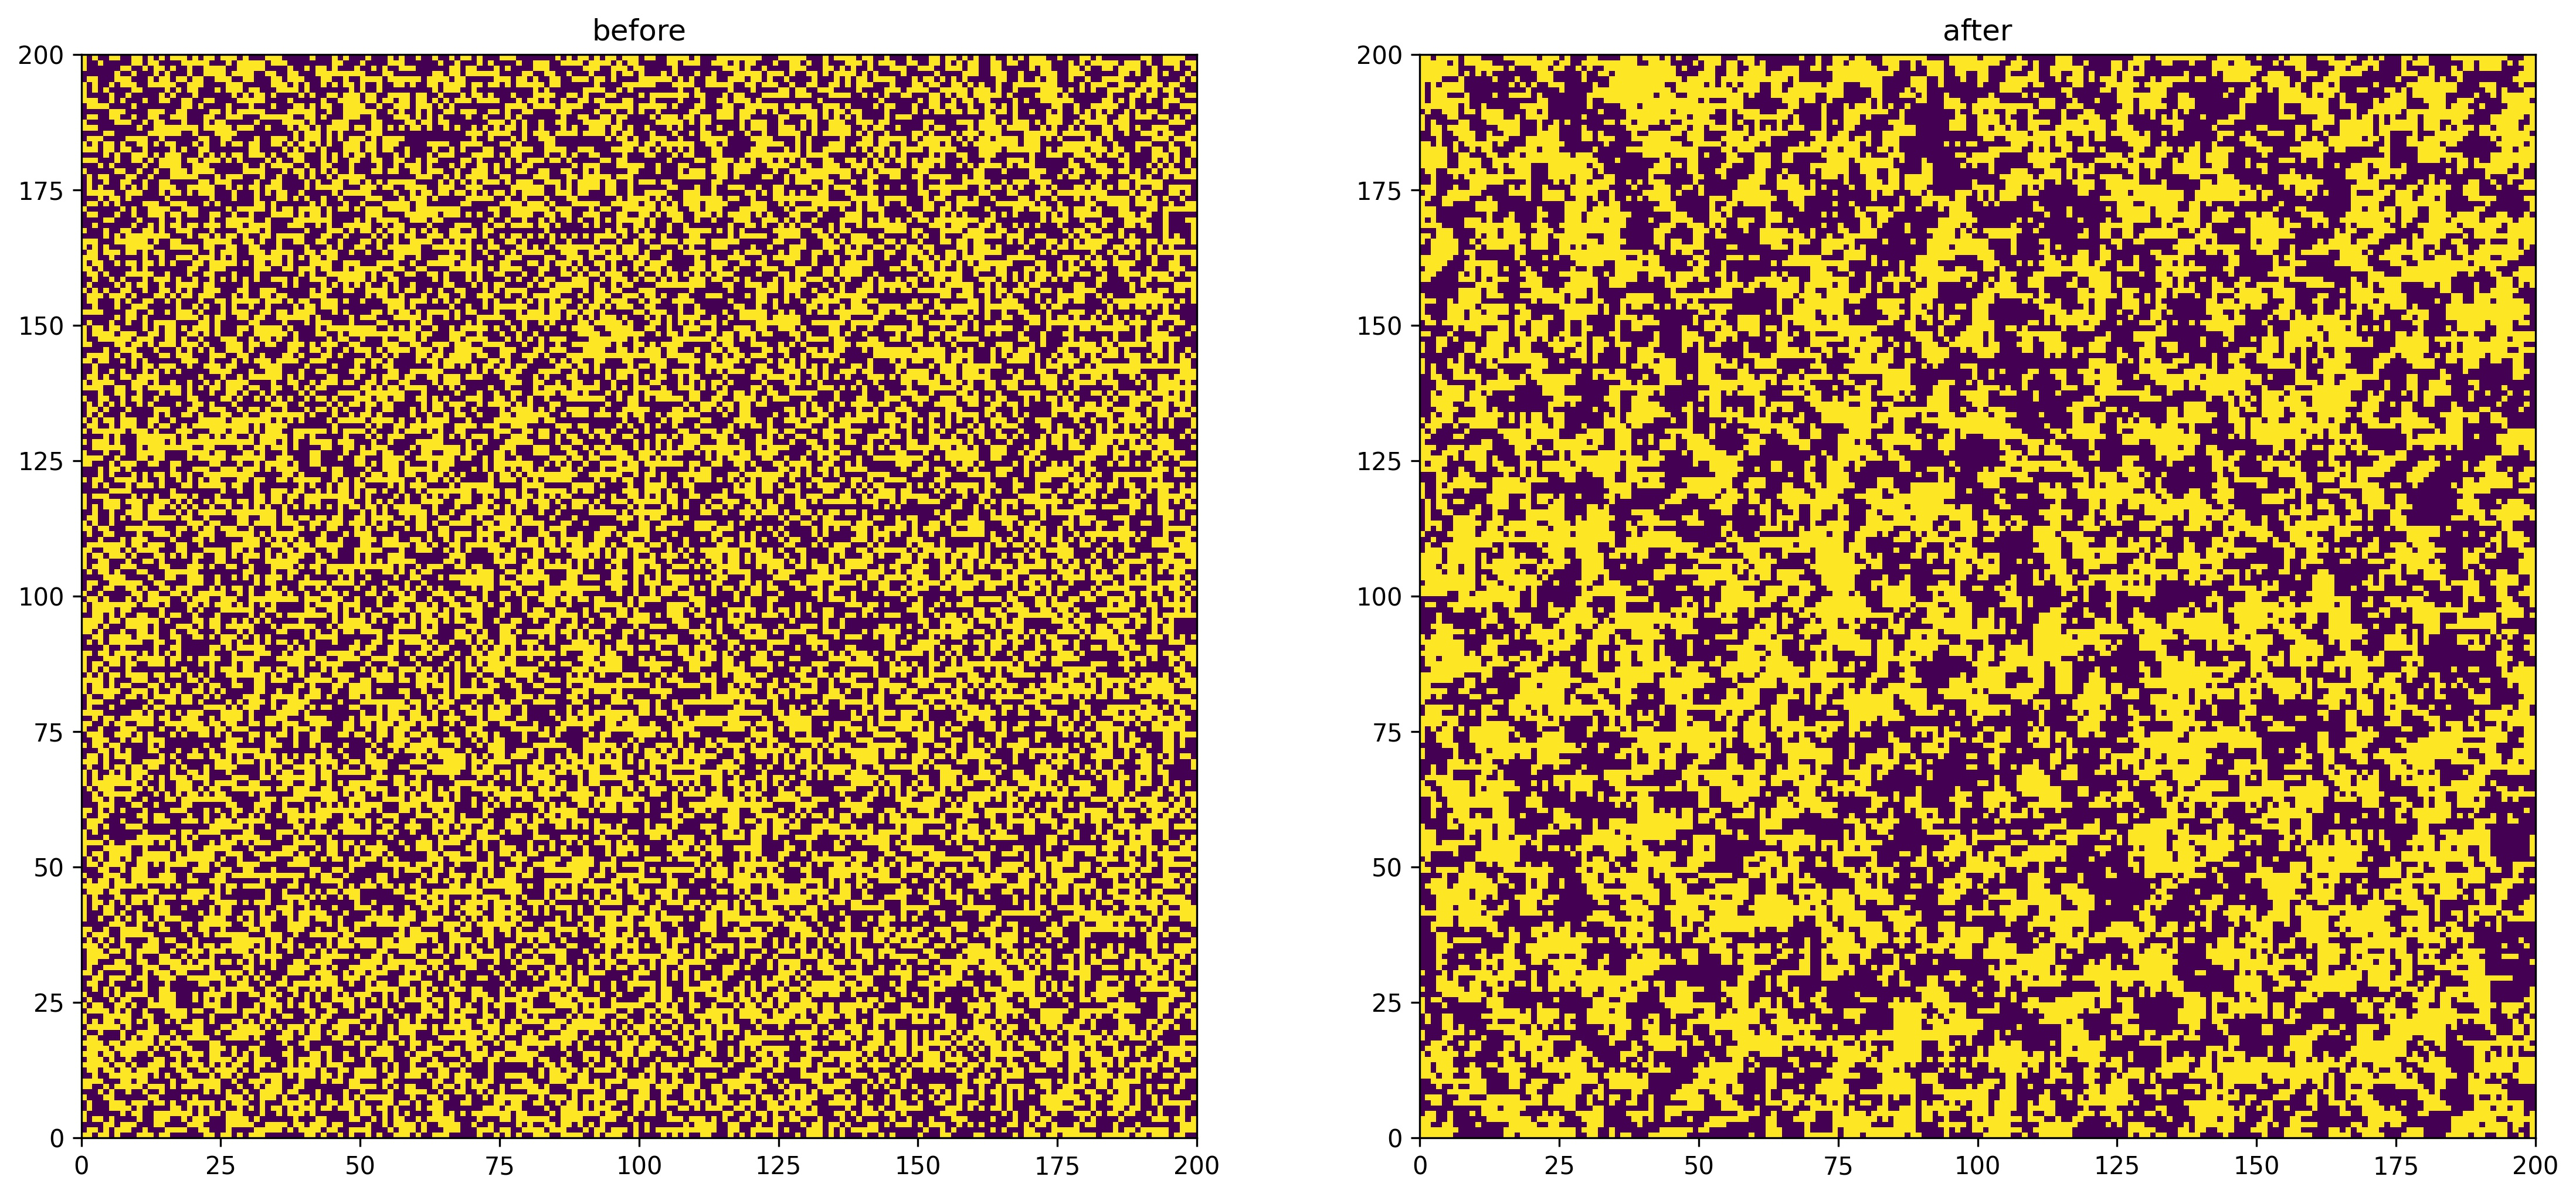
\includegraphics[width=0.9\linewidth]{../ba3.jpg}
		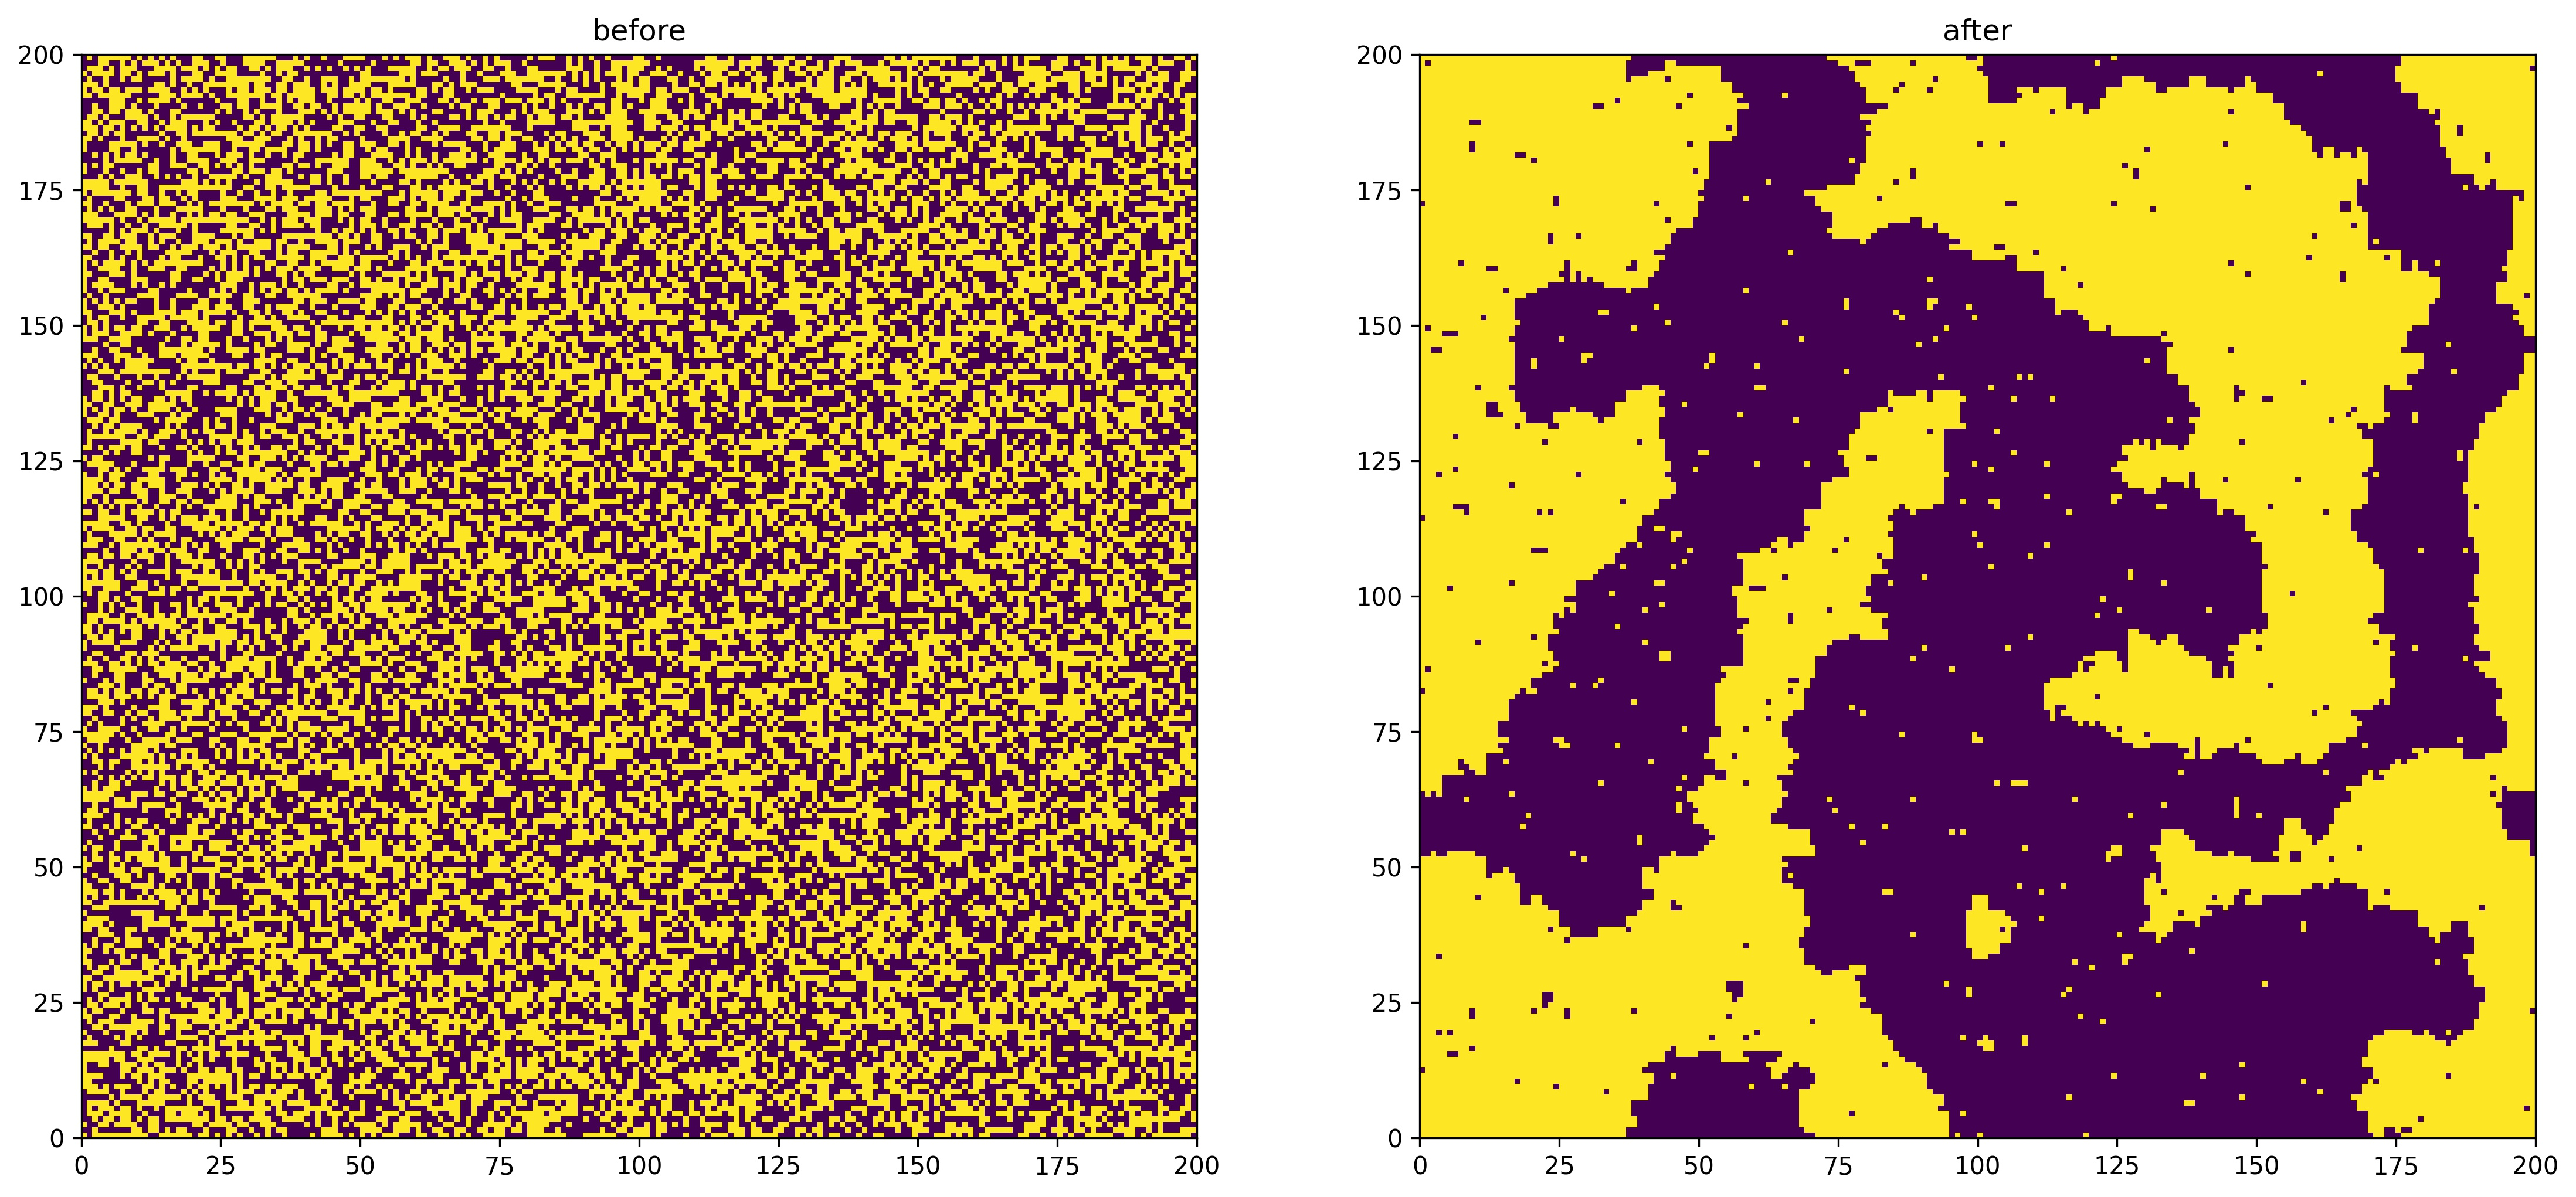
\includegraphics[width=0.9\linewidth]{../ba6.jpg}
		\label{fig:ising_grid}
		\caption{Ising model of size 200, before and after using the \texttt{metropolis()} function 200 times (top: $\beta = 0.3$, bottom: $\beta = 0.6$).}
	\end{figure}
	
	\section{Data Acquisition}
	In order to collect data from the system, first we need a method to check if the system has reached equilibrium. In order to do that, I made the method \texttt{equalize()} that uses 
	\texttt{metropolis()} $n = 100$ times and takes the energy samples along the process. Then checks if the auto-correlation of energies for a gap of $\frac{n}{10}$ is less that $e^{-3}$.
	If \texttt{True}, the system has reached equilibrium, otherwise repeat the process 100 more
	times and check for $n = 200$. and so on until we reach equilibrium.
	
	After the system has reached equilibrium, we need to take the auto-correlation of energies
	to see for how many steps our data are \emph{almost} not correlated to pick a sample.
	This is made possible using the \texttt{corr\_len()} function.
	Then, I pick the data in intervals of $h =$ \texttt{corr\_len(energies)}.
	
	This process is repeated for lengths $\{100, 110, 130, 160, 200\}$ and a linear space of 
	$\beta$ of size $40$, from $0.1$ to $0.7$ . I saved the data to CSV files and analyzed and 
	plotted them using the file \texttt{data\_analysis.ipynb}.\\
	The plots are available in Figs \ref{fig:data}
	\begin{figure}[h!]
		\centering
		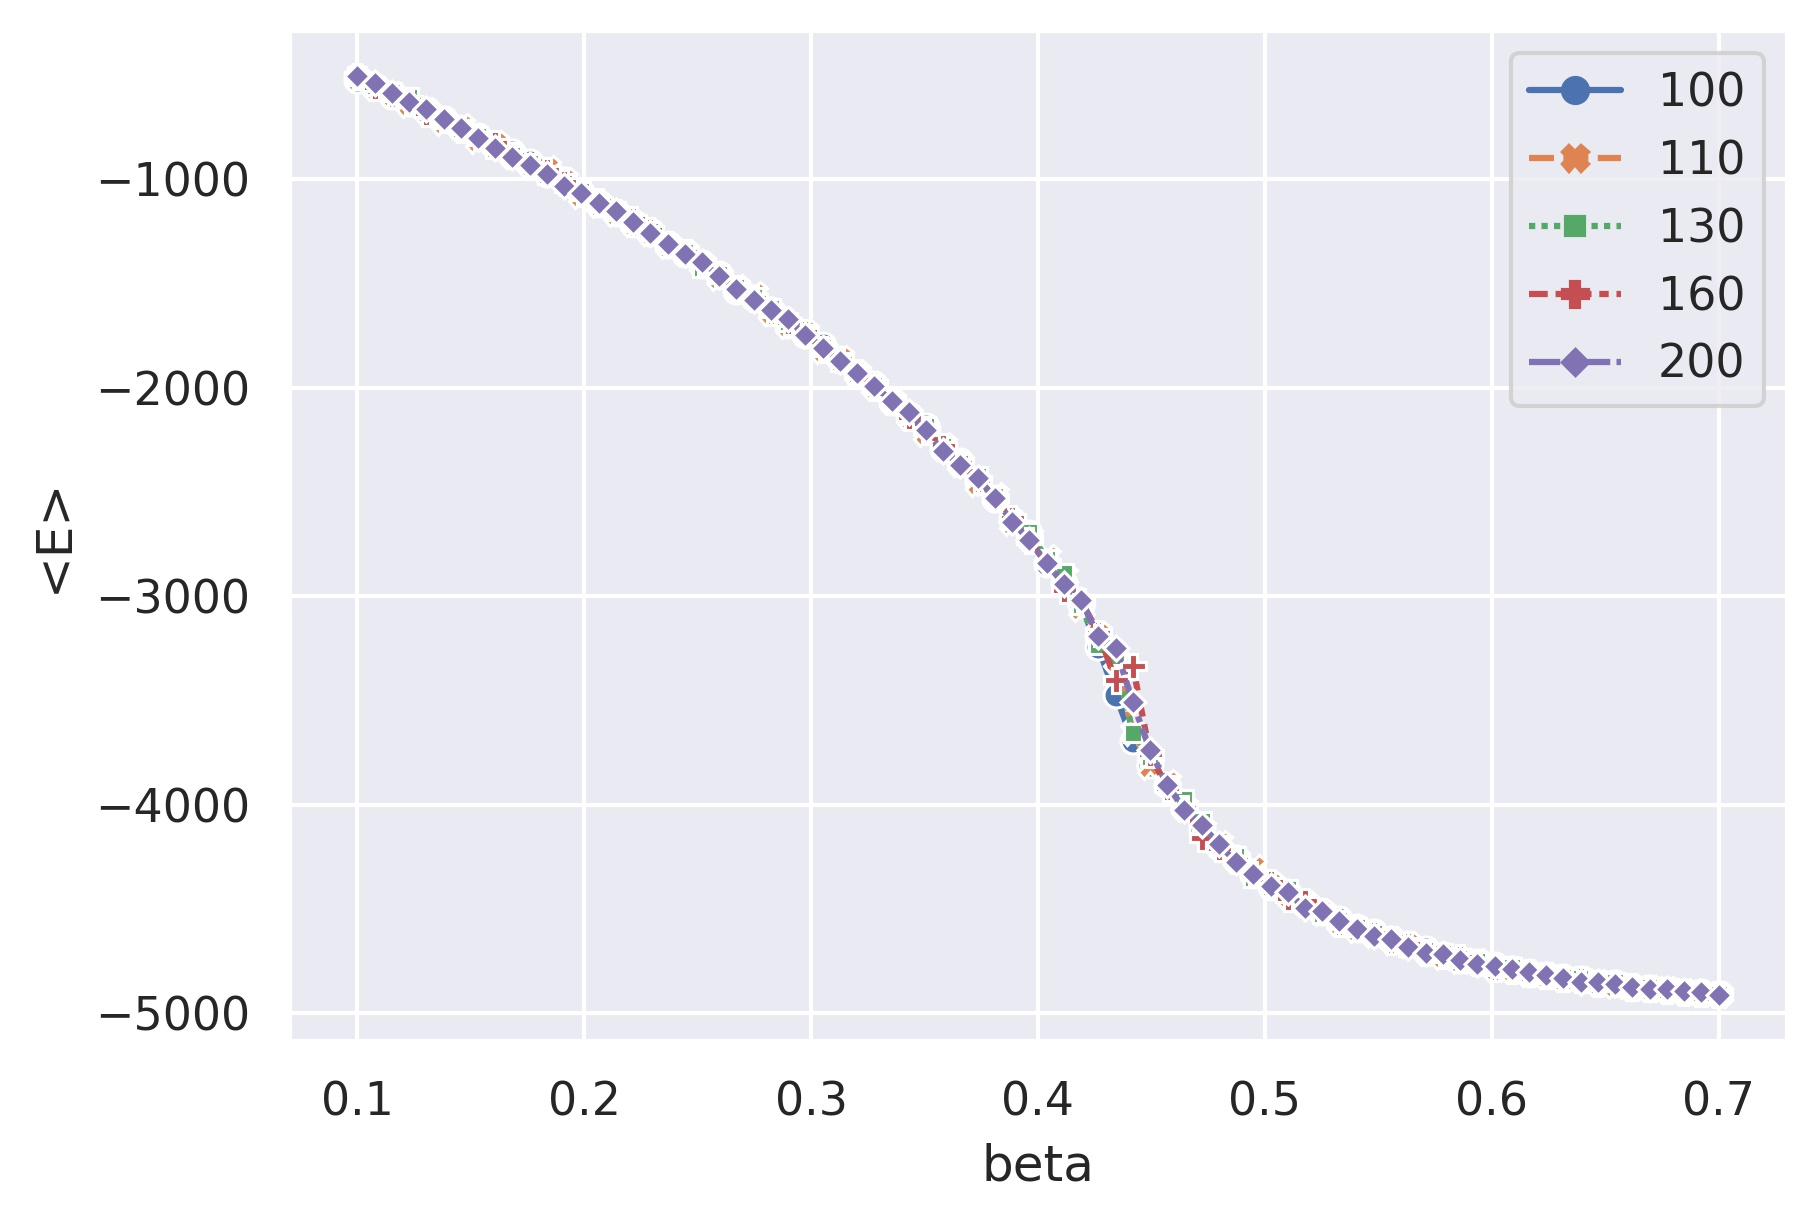
\includegraphics[width=0.45\linewidth]{../energy_plot.jpg}
		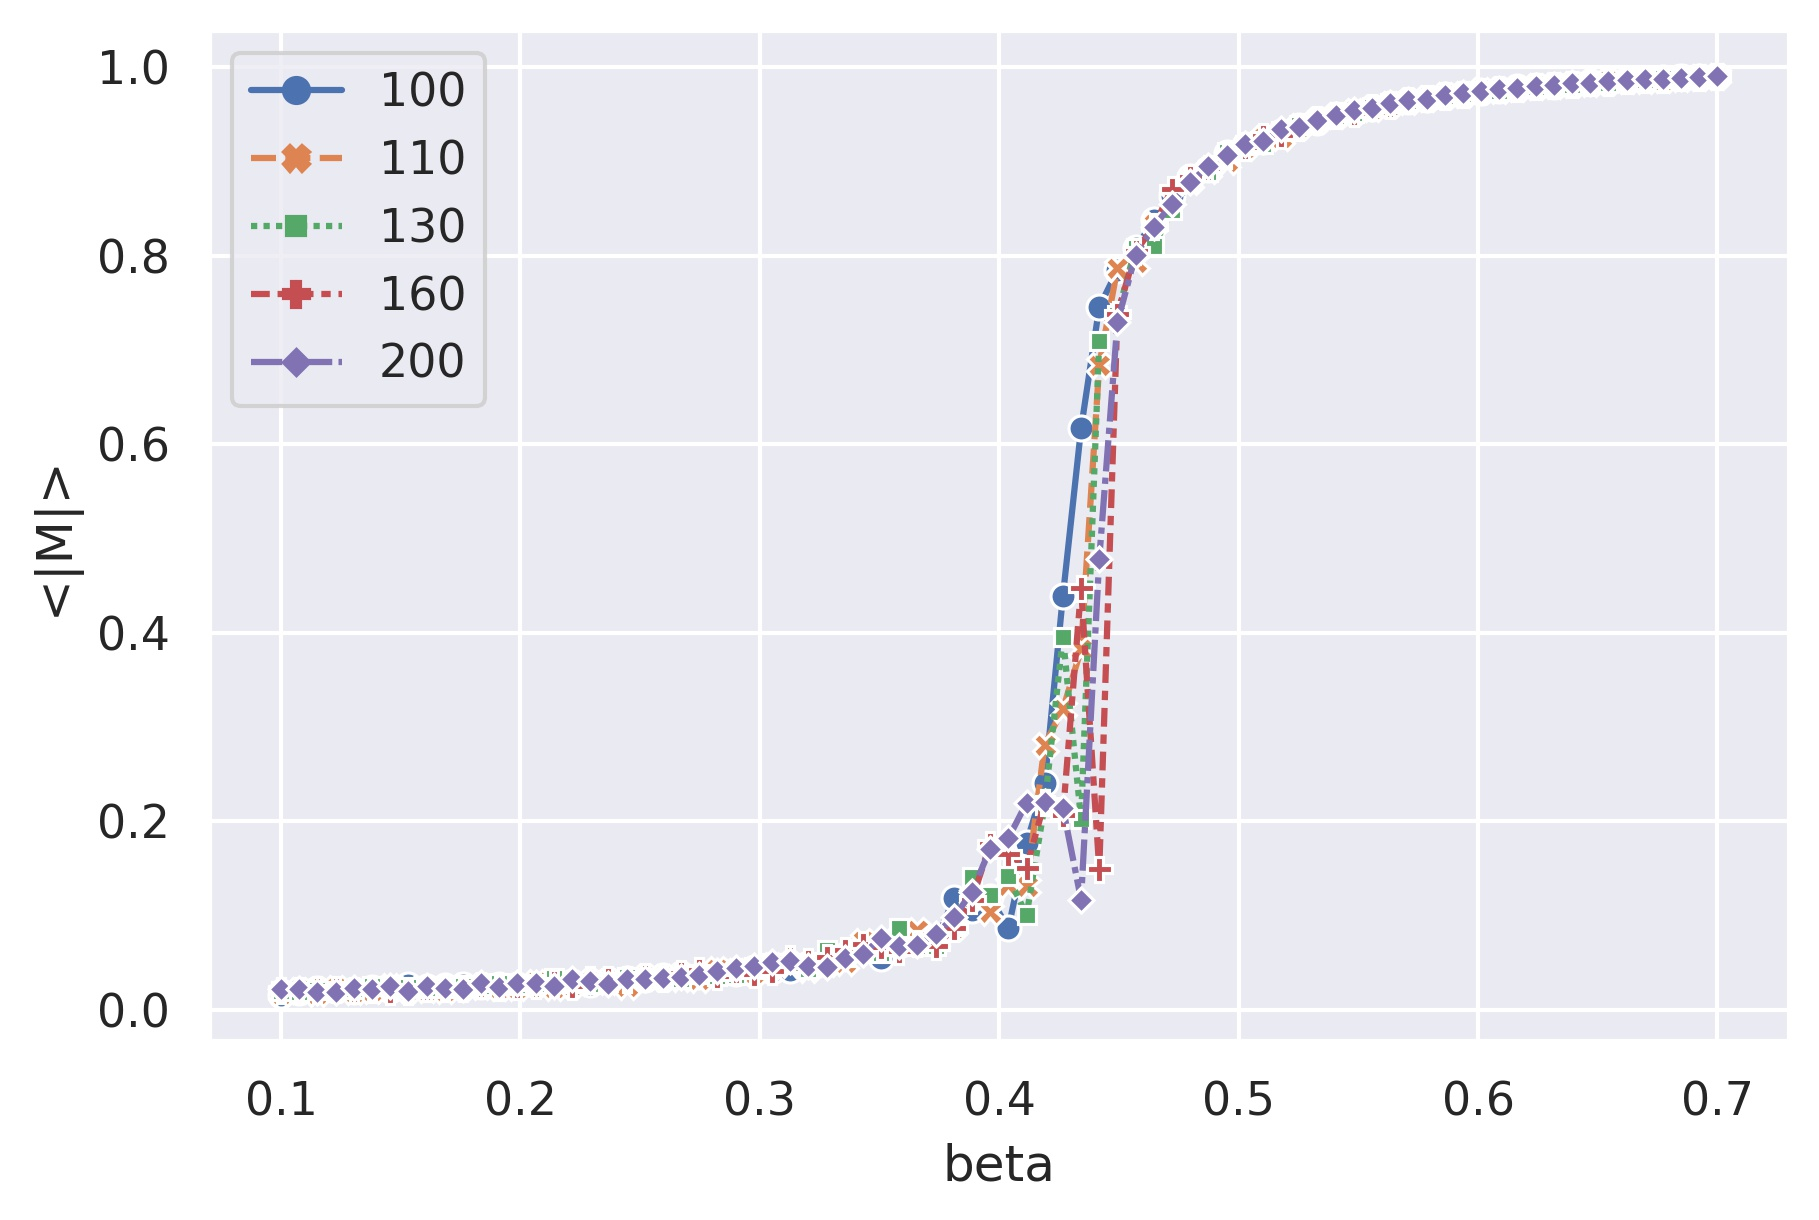
\includegraphics[width=0.45\linewidth]{../magnet_plot.jpg}
		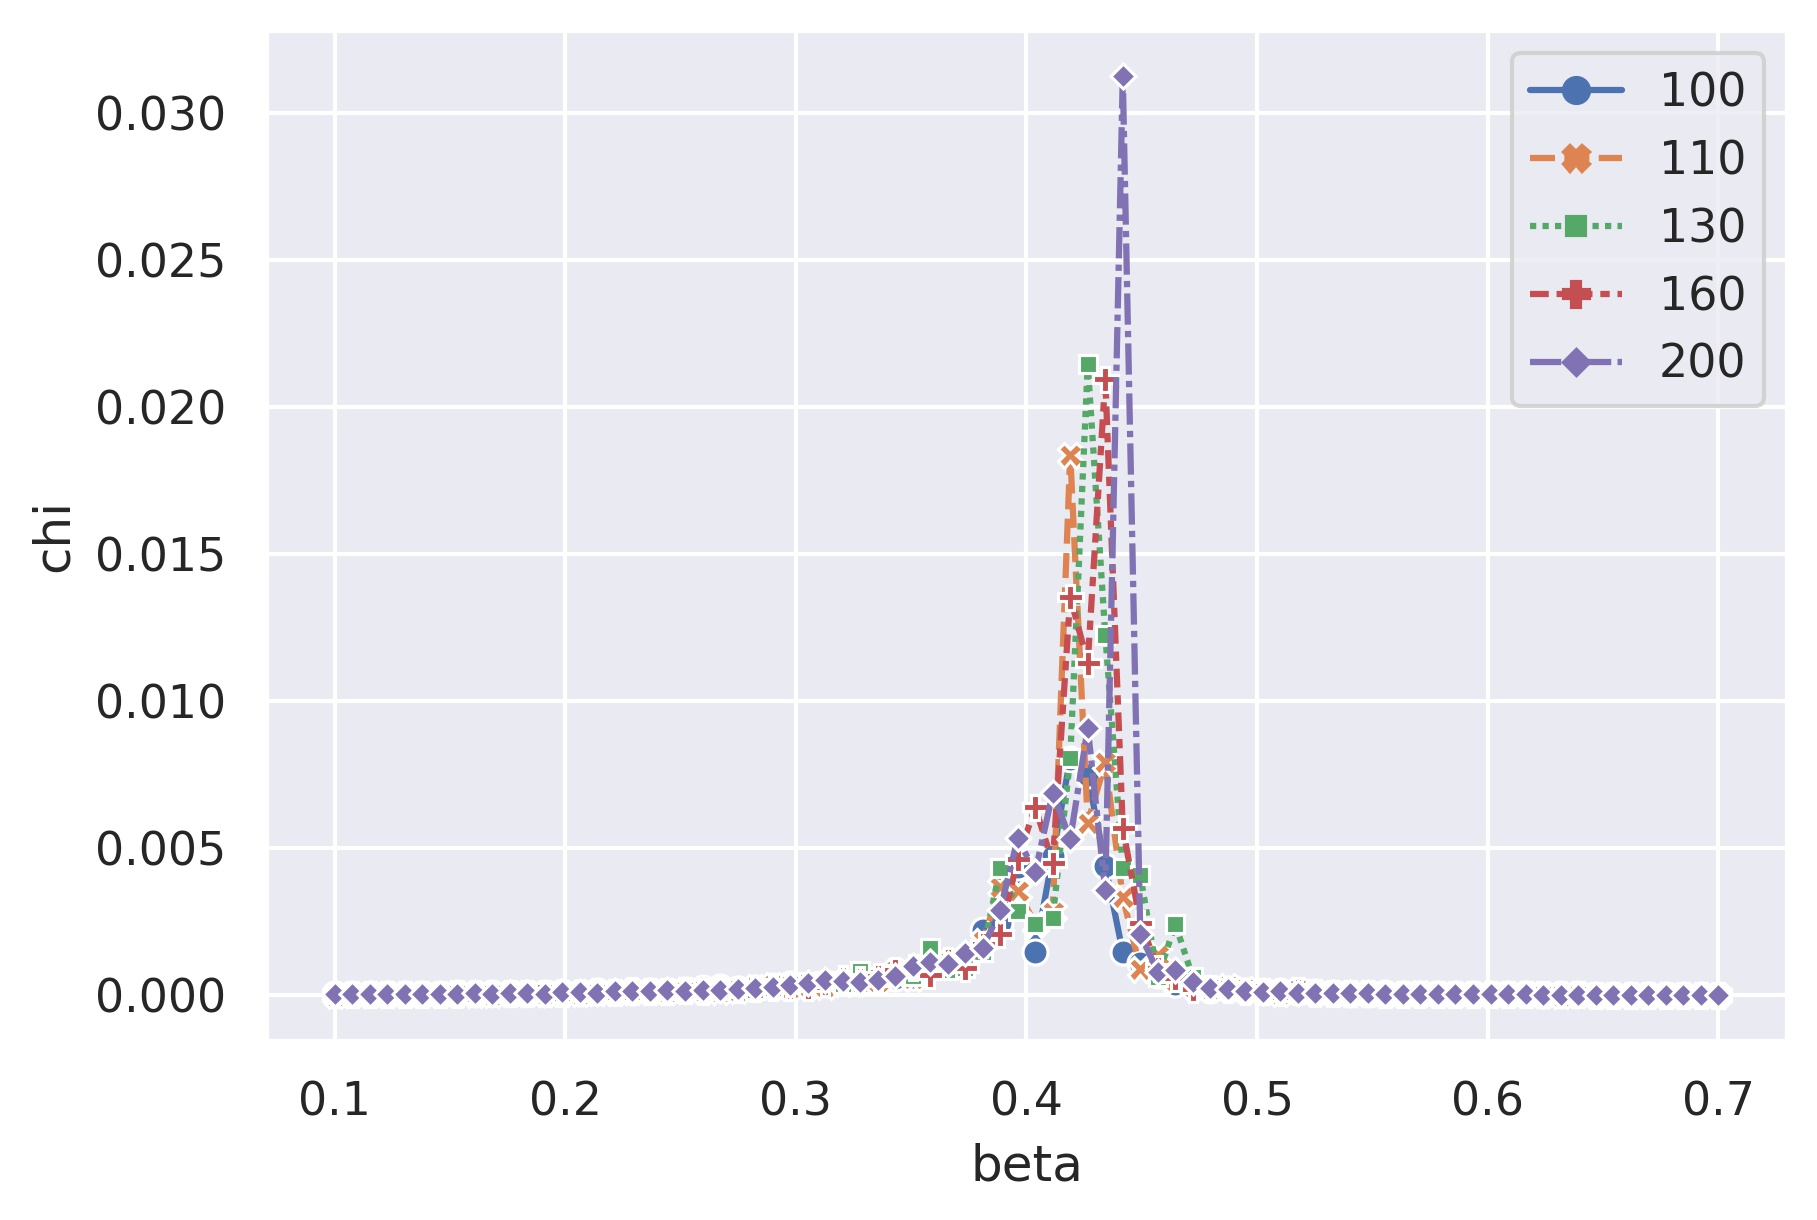
\includegraphics[width=0.45\linewidth]{../ksi_plot.jpg}
		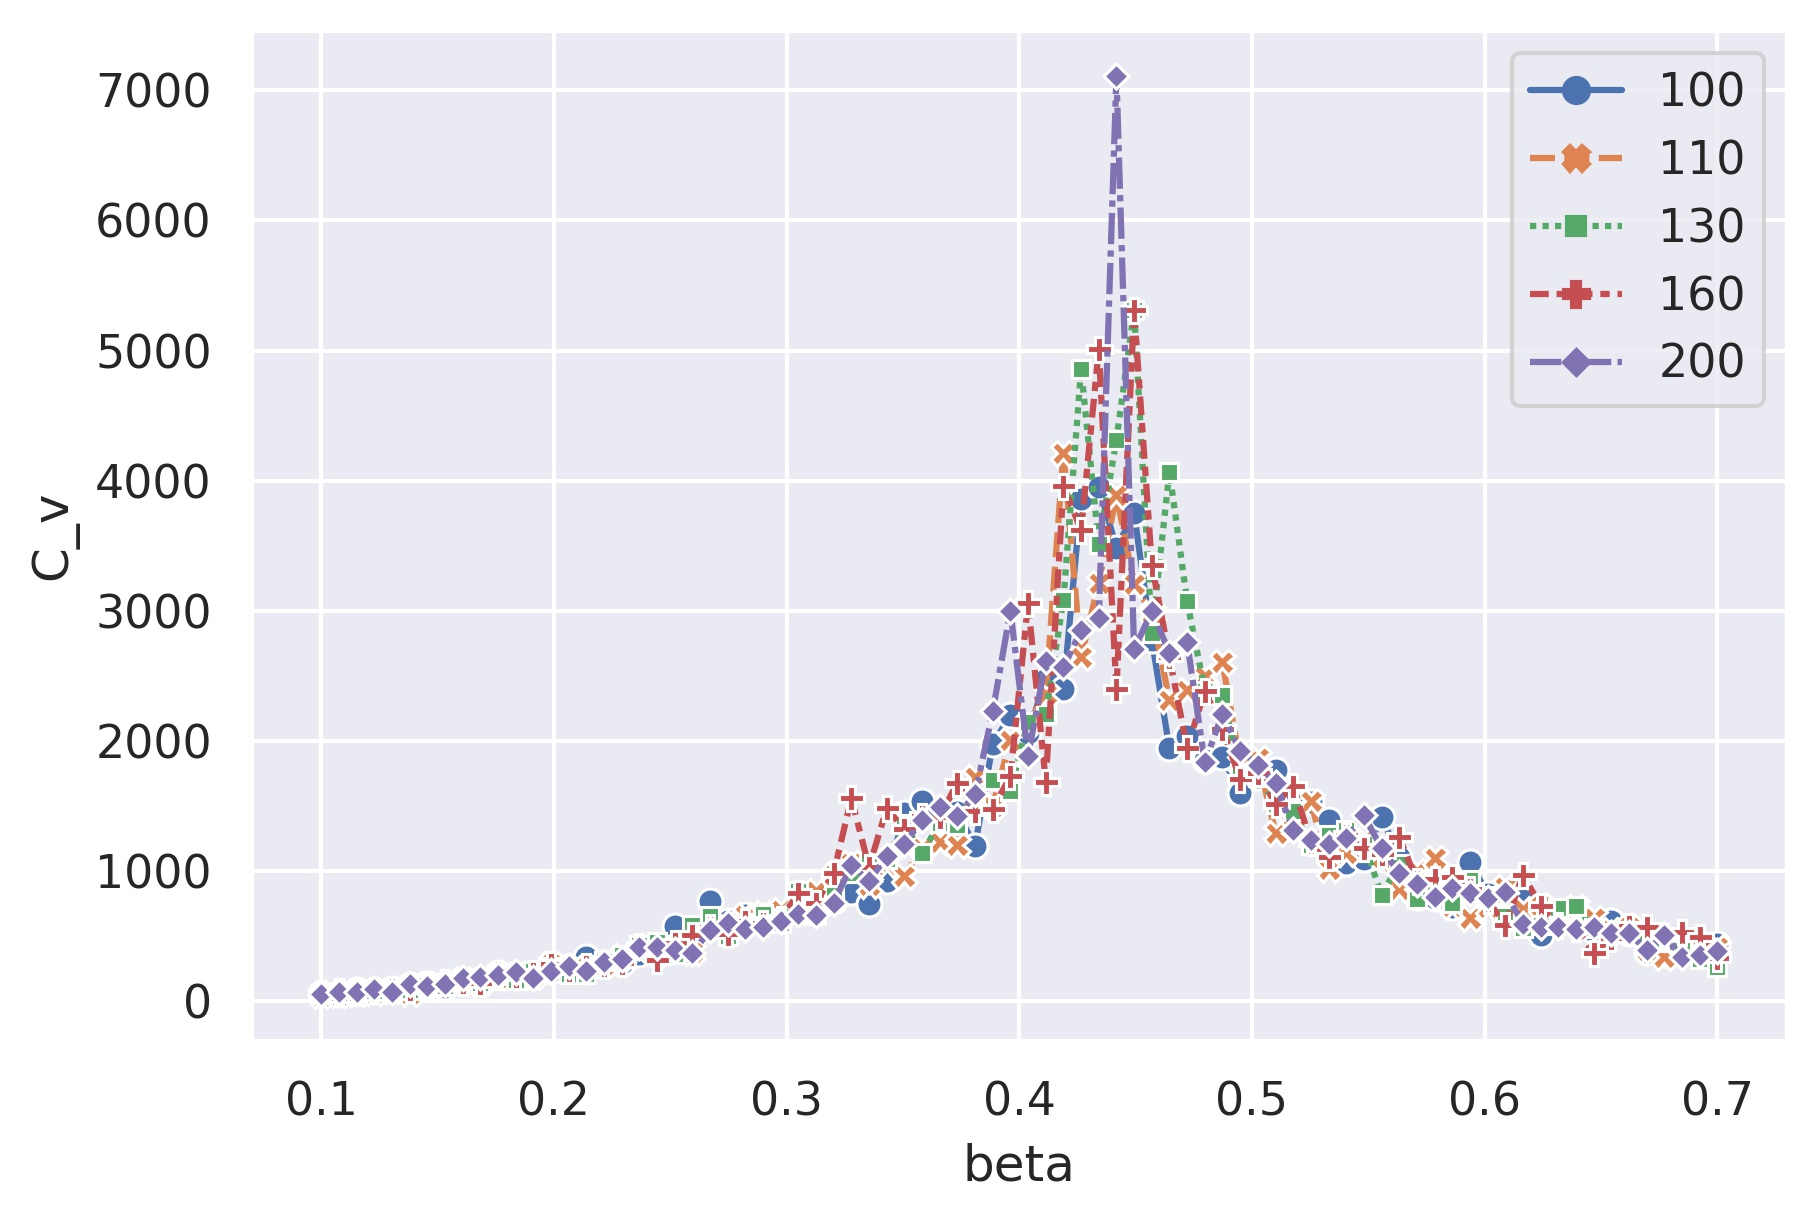
\includegraphics[width=0.45\linewidth]{../heat_cap_plot.jpg}
		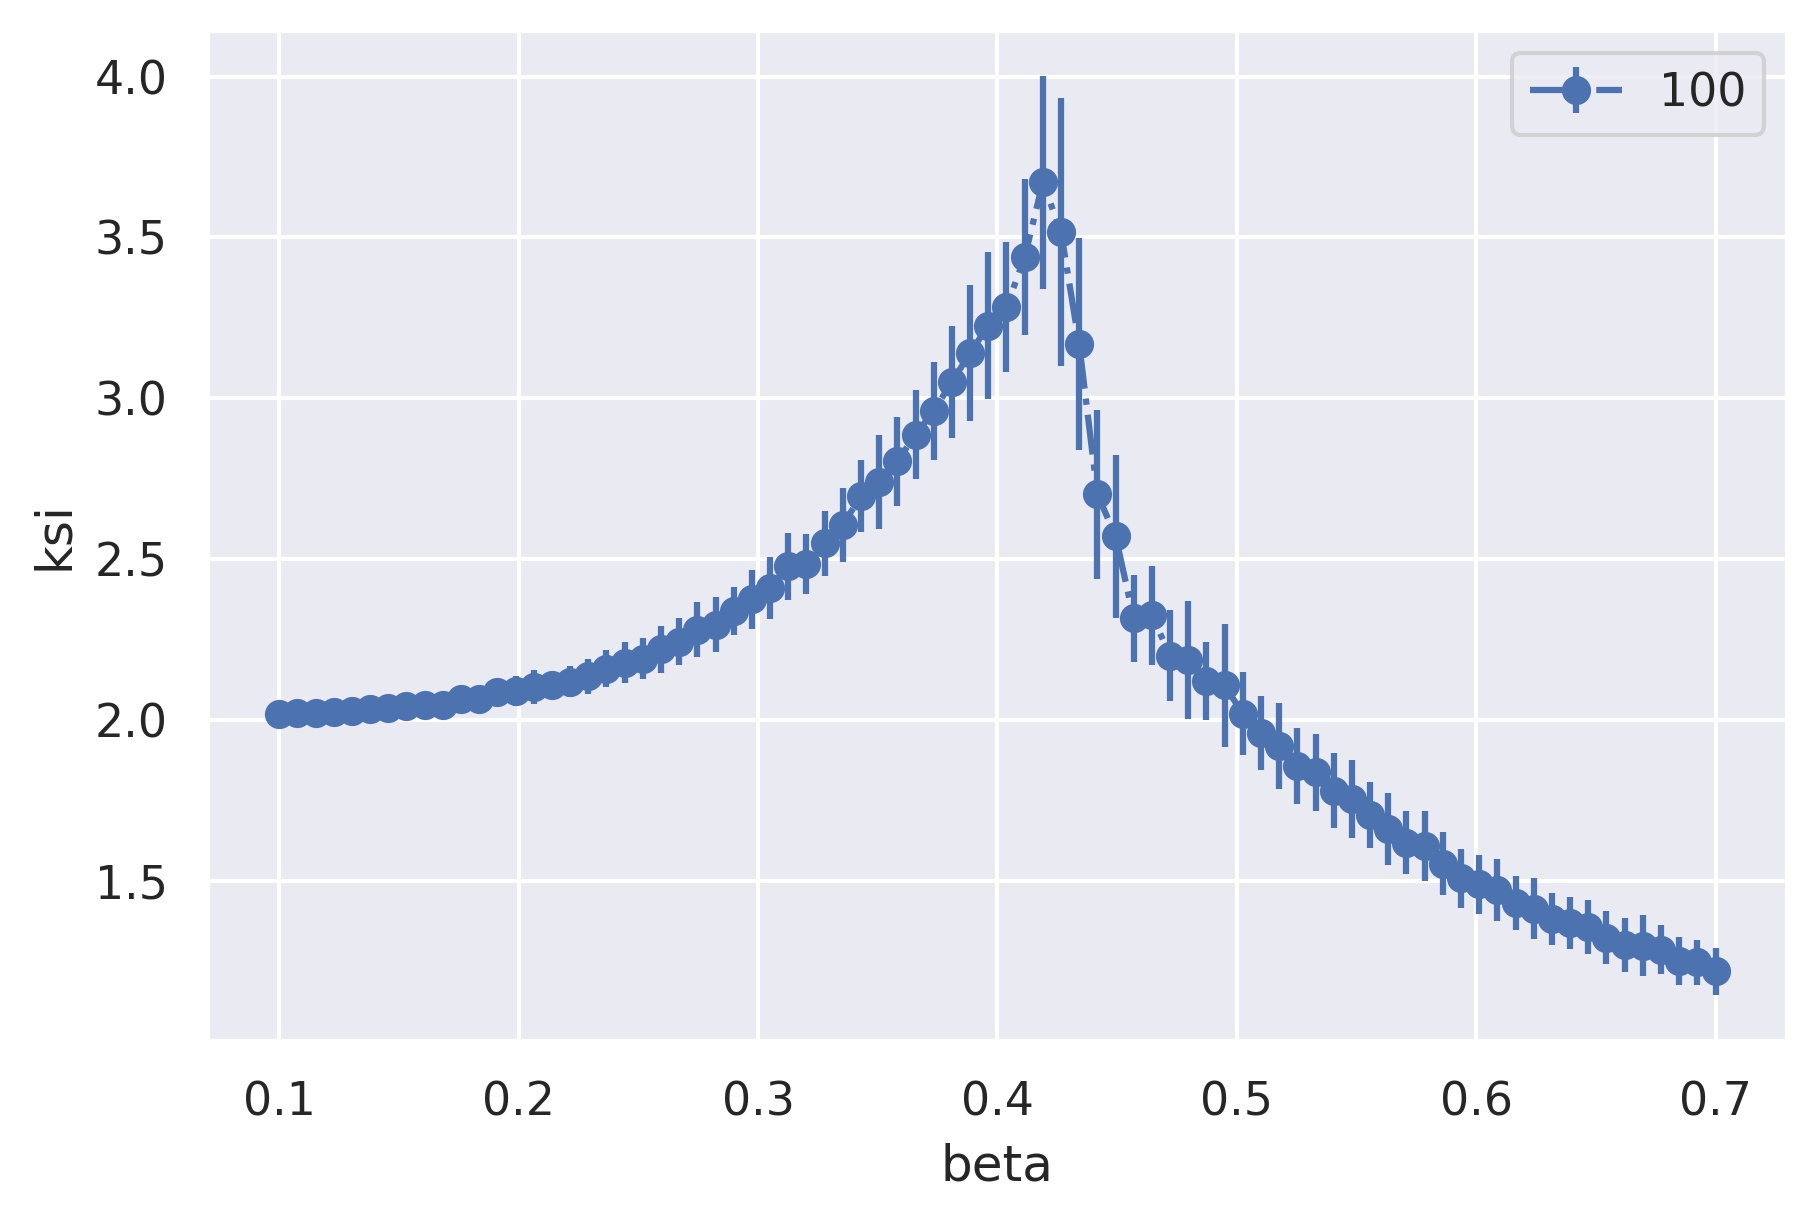
\includegraphics[width=0.45\linewidth]{../spin_cor_plot.jpg}
		\label{fig:data}
		\caption{Data vs. beta for $\beta$ from $0.1$ to $0.7$ and ising size in 
			$\{100, 110, 130, 160, 200\}$. from left to right and top down, we have \emph{energy}, \emph{magnetization}, \emph{ksi}, \emph{heat capacity}, $\xi$ \emph{only for $L = 100$}.}
	\end{figure}
	
	As for how I selected and changed the temperature, I started from high temp., 
	$\beta =\frac{1}{k_B T} = 0.1$ to $0.7$, and each time I was done taking data for each 
	$\beta$, I the equalized state of the system with the previous value of $\beta$ for the initial 
	condition of the system with new $\beta$. This way the necessary time to reach equilibrium is decreased and so is the risk of the system freezing.
	
	\section{Finding the critical exponents $\nu, \mu, \beta$ and the Coefficient $c_0$}
	The value for $c_0$ was found by fitting a log-log polynomial of degree 1 to the data. The function for $c_0$ is:
	\begin{equation}
		c_v = c_0 \ln(|T - T_c|), c_0 = 7.24 \pm 0.07
	\end{equation}
	
	For the other parameters since we have already shown the plots, we'll just report the numerical values here.
	\begin{equation}
	\begin{aligned}
		m &\sim L^{-\frac{\beta}{\nu}}, \qquad \beta = \pm \\
		\chi &\sim L^{-\frac{\gamma}{\nu}}, \qquad \frac{\gamma}{\nu} = - 1.49 \pm 0.56\\
		C_v &\sim L^{-\frac{\alpha}{\nu}}, \qquad \frac{\alpha}{\nu} = - 0.79 \pm 0.12\\
		\xi & \sim L^{-\frac{1}{\nu}}, \qquad \frac{1}{\nu} = 0.02\pm 0.08
	\end{aligned}
	\end{equation}

\end{document}